% ---
\chapter{Algoritmos de compressão sem perda}\label{cap:comp}
% ---

Os algoritmos de compressão podem ser categorizados em duas diferentes classes: os de compressão \textbf{com perda} e \textbf{sem perda}. 
Os \textbf{algoritmos de compressão com perda} admitem uma baixa porcentagem de perda de informações durante a codificação para obter maior performance, muito úteis na transmissão de dados em streaming por exemplo. 
Nos \textbf{algoritmos de compressão sem perda} o processo de codificação deve ser capaz de recuperar os dados em sua totalidade, geralmente utilizados em casos onde não pode haver perda de informações (como por exemplo, compressão de arquivos de texto).

Neste capítulo serão apresentados dois dos principais algoritmos de compressão sem perda (\textbf{Código de Huffman} e \textbf{Lempel-Ziv 77}), bem como algumas variações úteis para o propósito do presente trabalho.

\pagebreak

\section{Código de Huffman} \label{sec:huff}
O \textbf{algoritmo de Huffman} (desenvolvido por David Huffman em 1952 \cite{Huff}) é um dos componentes mais utilizados em algoritmos de compressão sem perda, servindo como base para algoritmos como o Deflate (utilizado amplamente na web).
Os códigos gerados a partir do algoritmos de Huffman são chamados \textbf{Códigos de Huffman}.

O código de Huffman é descrito em termos de como ele gera uma árvore
de código livre de prefixo com alfabeto código $W = \{0,1\}$. A árvore
é binária e assumimos rótulo $0$ nas arestas de um nó para um filho da
esquerda e rótulo $1$ nas arestas de um nó para um filho da direita.
Considere o conjunto de símbolos $M$ e, para cada símbolo $m_i\in M$,
seja $p_i$ a probabilidade associada a $m_i$.

\begin{algorithm}[H]
\caption{Algoritmo de Huffman} \label{alg:huff}
\begin{algorithmic}
	\State $Forest \gets \emph{[]}$\\
	\ForAll{$m_i \in M$} \Comment{Inicializando floresta}
		\State $T \gets newTree()$
		\State $node \gets newNode()$
		\State $node.weight \gets p_i$ \Comment{$w_i = p_i$}
		\State $T.root \gets node$
		\State $Forest.append(T)$ \Comment{Adiciona um nova árvore na floresta}
	\EndFor \\
	
	\While{$Forest.size > 1$}
		\State $T1 \gets ExtractMin(Forest)$ \Comment{Retorna a árvore cuja raiz é mínima, e retira da floresta}
		\State $T2 \gets ExtractMin(Forest)$
		\State $HTree \gets newTree()$
		\State $HTree.root \gets newNode()$ \\
		\State $HTree.root.left \gets T1.root$
		\State $HTree.root.right \gets T2.root$
		\State $HTree.root.weight \gets T1.root.weight + T2.root.weight$
		\State Forest.append(HTree) 
	\EndWhile
\end{algorithmic}
\end{algorithm}

\subsection{Análise assintótica}

Seja $n$ o tamanho do conjunto de símbolos $M$. Para que o algoritmo percorra toda a floresta, formada por uma árvore para cada $m \in M$, serão necessárias $n$ iterações. Considerando que as funções \emph{ExtractMin()} e \emph{.append()} foram construídas a partir de uma fila de prioridades de \textbf{heap} e essas operações podem ser realizadas em tempo $O(\log_2 n)$, o algoritmo será executado em tempo $O(n\log_2 n)$ \cite{Ble}.

\subsection{Corretude}
O teorema a seguir (escrito por Huffman, 1952 \cite{Huff}) afirma
que os códigos de Huffman minimizam o comprimento médio, ou seja, são
ótimos dentre os códigos livres de prefixo.

Nesta seção, considere um alfabeto de origem $M = \{m_1,\dotsc, m_n\}$
com probabilidade $p_i$ para cada símbolo~$m_i$ e alfabeto código $W =
\{0,1\}$. Dizemos que um código $C: M\to W^+$ livre de prefixo é
\textbf{ótimo} se $l_a(C) \leq l_a(C')$ para todo código $C': M\to
W^+$ livre de prefixo.

\begin{theorem}
  \label{thm:otimo_huffman}
  Seja $C_{H}$ um código gerado pelo algoritmo de Huffman. Temos que
  $C_{H}$ é ótimo.
\end{theorem}

Antes de provar o teorema, começamos com uma simples observação.
  
\begin{lemma} \label{lemma:dist_prob_avg_size} Seja $C:M\to W^+$ um código livre de prefixo ótimo. Para todo $i,j \in\{1,\dotsc, n\}$, se $p_i > p_j$, então $l(C(m_i)) \leq l(C(m_j))$
\end{lemma}
  \begin{proof}
    Sejam $i,j \in\{1,\dotsc, n\}$ e suponha que $p_i > p_j$.  Seja
    $w_i = C(m_i)$ e seja $w_j = C(m_j)$. Para efeito de contradição,
    assuma que $l(w_i) > l(w_j)$.  Agora construa um novo código $C'$,
    trocando $w_i$ por $w_j$. Ou seja, $C'(m_k) = C(m_k)$ para todo $k
    \in \{1,\dotsc, n\} \setminus \{i,j\}$, $C'(m_i) = w_j$ e $C'(m_j)
    = w_i$.  Dado o comprimento médio $l_a(C')$ é
 \begin{align*}
   l_a(C') &= l_a(C) + p_j\cdot(l(w_i) - l(w_j)) + p_i\cdot(l(w_j) - l(w_i)) \\
   &= l_a(C) + (p_j - p_i)(l(w_i) - l(w_j))\\
   &< l_a(C),
 \end{align*}
 pois $p_j - p_i < 0$ e $l(w_i) - l(w_j)>0$. Isso contradiz o fato do
 código $C$ ser ótimo.
  \end{proof}

\noindent \textbf{Nota:} Perceba que em uma árvore de Huffman, o comprimento de uma palavra-código também representa seu nível na árvore.

\begin{proof}[Prova do Teorema~\ref{thm:otimo_huffman} (Blelloch, 2013 \cite{Ble})]
A prova se dará por indução sobre o tamanho $n$ de $M$. Para a base,
tome $n=2$. Nesse caso, o resultado é trivialmente verdadeiro
considerando que o algoritmo de Hufman gera um código que atribui um
bit pra cada símbolo de~$M$. Assuma então que $n>2$ para o passo
indutivo. Sejam $x$ e $y$ nós associados a símbolos $m_a$ e $m_b$
respectivamente tais que $p_a \leq p_b \leq p_i$ para todo $i \in
\{1,\dotsc,n\}\setminus\{a,b\}$. Ou seja, $x$ e $y$ poderiam ser os nós escolhidos como o primeiro par pelo algoritmo de Huffman.

Seja $m'$ um novo símbolo com probabilidade $p_a+p_b$ e seja $M' =
(M\cup\{m'\})\setminus\{m_a, m_b\}$. Note que $|M'| < n$. Seja $T'$
uma árvore obtida pelo algoritmo de Huffman para $M'$. Por hipótese de
indução o código $C'$ da árvore $T'$ é ótimo para $M'$. A árvore $T$
obtida pelo algoritmo de Huffman é a árvore $T'$ adicionando os nós
$x$ e $y$ como filhos do nó associado a $m'$. Seja $C$ o código da
árvore $T$.

Agora iremos comparar com um código ótimo. Afirmamos que
\begin{equation}
 \label{irmaos}
\text{Existe um código $C^*$ livre de prefixo ótimo com árvore $T^*$
  tal que $x$ e $y$ são \textbf{irmãos}.}
\end{equation}
Seja $z$ o pai de $x$ e de $y$ em $T^*$. Note que a árvore obtida a
partir $T^*$ pela remoção de $x$ e $y$ e associando $z$ ao símbolo
$m'$ (de probabilidade $p_a+p_b$) gera um código $C^{**}$ para $M'$. Pela
otimalidade de $C'$, temos que
\begin{equation*}
  l_a(C^*)
  =
   l_a(C^{**})+p_a+p_b
  \geq
  l_a(C')+p_a+p_b
  =
  l_a(C),
\end{equation*}
o que mostra a otimalidade de $C$.


Finalmente provamos a afirmação em~\eqref{irmaos}.  Dado um código
$C''$ livre de prefixo ótimo com árvore $T''$, pelo
lema~\ref{lemma:dist_prob_avg_size}, sabemos que os símbolos com as
menores probabilidades estão nos menores níveis de $T''$ (ou seja,
associados a palavras-código de maior comprimento). Portanto, $x$ e
$y$ são folhas em $T''$. Seja $w \in\{x,y\}$ tal que $w$ é $x$ se o
nível de $x$ é menor ou igual ao nível de $y$ e seja $v$ o nó em
$\{x,y\}\setminus\{w\}$. (Note que $w$ só pode ser $y$ no caso em que
$p_a = p_b$, pelo lema~\ref{lemma:dist_prob_avg_size}). Seja $z$ o pai
de $w$. Se $w$ é o único filho de $z$, então poderíamos mudar $w$ para
$z$ (pois $z$ não é associado a nenhum símbolo dado que $C''$ é livre
de prefixo). Portanto, $w$ tem um nó \textbf{irmão} $w'$. Se $w'$ não
é $v$, trocar $w'$ com $v$ gera um código de comprimento menor ou
igual ao de $C''$ pelo lema~\ref{lemma:dist_prob_avg_size}. 
\end{proof}


\section{Lempel-Ziv 77 (LZ77)}

\subsection{Algoritmos de Lempel-Ziv}
Nos anos de 1977 e 1978, Jacob Ziv e Abraham Lempel publicaram dois artigos apresentando os algoritmos \textbf{LZ77} e \textbf{LZ78} \cite{LZ}, que serviriam como base para uma família de algoritmos de compressão (conforme mostrado na Figura~\ref{fig:lz77}), chamados de algoritmos de \textbf{Lempel-Ziv}.
Os algoritmos de Lempel-Ziv realizam o processo de compressão baseado em um \textbf{dicionário} de mensagens vistas anteriormente (diferente do \nameref{alg:huff}, que utiliza a probabilidade associada a cada símbolo). 
Tanto o LZ77 quanto o LZ78 têm um funcionamento parecido, que se resume em substituir partes da entrada por referências a partes iguais anteriormente processadas, e diferem na maneira em que procuram por repetições a serem substituídas. 

\begin{figure}[h]
   \centering
   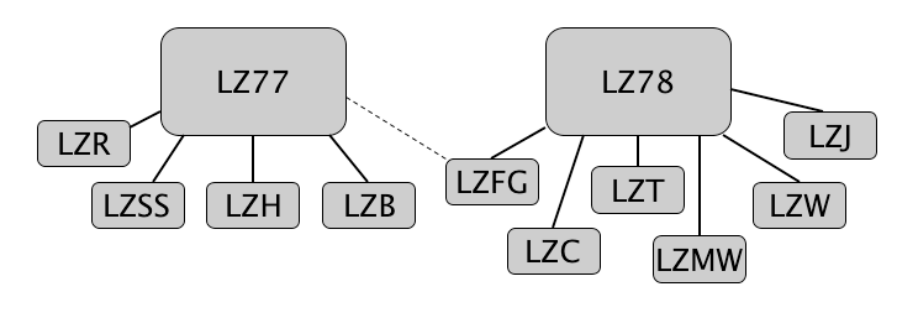
\includegraphics[scale=0.75]{figs/lz77fam.png}
    \caption{Familia de algoritmos Lempel Ziv}
    \label{fig:lz77}
 \end{figure}

\subsection{Descrição do LZ77}
O LZ77 e suas variações utilizam a técnica de \emph{janela deslizante} para encontrar mensagens correspondentes. 
A janela é dividida em duas partes separadas por um \emph{cursor} (que se move conforme novas mensagens são codificadas).

A mensagem à esquerda do cursor é chamada de \textbf{dicionário}, e contém todos os símbolos já codificados. Já a mensagem à direita do \emph{cursor} é chamada de \textbf{lookahead buffer}.
A ideia geral do algoritmo é substituir as mensagens do \emph{lookahead buffer} por \textbf{tokens}, onde cada \emph{token} é constituído por uma \emph{tupla} que ``aponta''  para a maior mensagem correspondente a cadeia no início do \emph{lookahead buffer}.

A \emph{tupla} que constitui os \emph{tokens} é formada por três valores:
um valor inteiro que indica quantas posições para trás o \emph{cursor} deve retornar até encontrar o início da cadeia, 
um segundo valor inteiro indicando o tamanho da cadeia,
e um caracter (preenchido com $m_{cursor}$ ou $null$ para \textbf{tokens não vazios}).

Os \emph{tokens} podem ser vazios, quando não encontramos nenhuma mensagem correspondente, neste caso, os dois primeiros valores da \emph{tupla} são preenchidos com zeros.
Por exemplo, se durante a compressão de um texto encontrássemos o símbolo ``a'' pela primeira vez (isso é, não existe correspondência pra ele no \emph{dicionário}), a saída seria o \emph{token vazio} $(0, 0, $``a''$)$.

\begin{algorithm}[H]
\caption{Algoritmo Lempel-Ziv 77} \label{alg:lz77}
\begin{algorithmic}

	\State $cursor \gets 0$
	\State $tokens \gets []$

	\While{$cursor < M.size()$}
		\State $position, len \gets findLongestMatch(M, cursor)$ \Comment{Retorna a posição e tamanho da maior cadeia correspondente}
		\If{$len > 0$} \Comment{Cria novo token, que aponta para a cadeia encontrada}
			\State $tokens.append([position, len, null])$
			\State $cursor \gets cursor + len$
		\Else
			\State $tokens.append((0, 0, M[cursor]))$ \Comment{Token vazio}
			\State $cursor \gets cursor + 1$
		\EndIf
	\EndWhile
\end{algorithmic}
\end{algorithm}

\subsection{Função ``\emph{findLongestMatch}'' }
O \emph{LZ77} possui um processo de decodificação muito eficiente, porém consome muitos recursos computacionais na codificação. 
Isto é, ele é mais eficiente para casos onde pretende-se decodificar o arquivo múltiplas vezes, ou ainda decodificá-lo numa máquina com menor poder computacional. 
O ``gargalo'' da compressão está na técnica de busca pelo \emph{dicionário} para encontrar a mensagem correspondentes mais longa.

O método convencional utilizado é a \textbf{busca linear}, que consiste em comparar cada posição no dicionário com o \emph{lookahead buffer} e selecionar a maior correspondência encontrada. 
Tome $N$ como o tamanho do dicionário e $M$ como o tamanho do \emph{lookahead buffer}, no pior caso, a busca linear é realizada em tempo $O(NM)$. 
A busca será executada $M + N$ vezes, isto é, a complexidade geral do algoritmo é $O( N^{2}M + M^{2}N)$.

\subsection{Melhorias na performance da função ``\emph{findLongestMatch}'' }

Uma das possíveis abordagens para melhorar a busca linear é utilizar estruturas de dados auxiliares, que indexam os símbolos do dicionário para tornar a busca mais rápida.
Bell (1993) \cite{TD}  testa diferentes estruturas de dados (árvores trie, hash tables, árvores binárias de busca entre outros). 
Para este trabalho utilizaremos a \textbf{lista ligada} como estrutura de dados auxiliar (principalmente por possuir uma implementação mais simples). 

Para construir uma estrutura de dados auxiliar com lista ligada, podemos criar uma lista para cada símbolo no dicionário, que contenha os índices onde o símbolo pode ser encontrado.  
Para limitar a janela de busca, podemos construir a lista como uma \emph{fila}, onde ao atingirmos a capacidade máxima da janela de busca, removemos o menor índice (que estaria no início da fila). 
Note que, o tamanho máximo da lista depende da quantidade de bits que queremos utilizar para construir o \emph{token}.

Encontramos a maior mensagem correspondente, comparando o \emph{lookahead buffer} com as cadeias de símbolos iniciadas a partir de índices contidos na lista que corresponde ao primeiro símbolo do \emph{lookahead buffer}.
Neste contexto, o pior caso ocorrerá quando todos os símbolos no dicionário forem iguais, pois todas as posições no dicionário seriam checadas (levando a uma performance equivalente a da busca linear).
Entretanto, para uma base de dados de texto real com grande quantidade de dados isso raramente acontece, e apenas uma quantidade $K \ll N$ de possíveis mensagens são realmente checadas.

\section{Compressão baseada em palavras}
A implementação padrão para a maioria dos algoritmos de compressão utiliza como \emph{alfabeto de origem} elementos de 8 bits (também conhecidos como \textbf{\emph{caracteres}}).
Tal método limita a correlação de cadeias mais longas, e tem sua eficiência limitada quando aplicado a grande quantidade de dados. 
Em contrapartida, se definirmos cada símbolo do \emph{alfabeto de origem} como uma sequência caracteres, poderíamos tirar vantagem de longas correspondências e talvez obter melhores resultados na compressão.

Quando a natureza dos dados é previamente conhecida, podemos tomar vantagem da sua estrutura para definir os símbolos de uma maneira mais eficiente. 
Em especial, linguagens ``faladas'' possuem uma estrutura hierárquica bem definida, que vai desde o agrupamento de letras em sílabas, silabas em palavras, palavras em frases e assim por diante. 

Neste contexto, definiremos uma \textbf{\emph{palavra}} como uma sequência maximal de \emph{caracteres} alfanuméricos, divididos por sequências de caracteres não alfanuméricos chamados \emph{separadores} (baseado na definição feita por Bentley (1986) \cite{Bentley}).
A compressão baseada em palavras é uma modificação dos algoritmos de compressão clássicos, que considera cada palavra como um símbolo (i.e, o \emph{alfabeto de origem} passa a ser composto por \emph{palavras}, não por \emph{caracteres}).

\subsection{Huffword} \label{sub:huffw}
O método de compressão \emph{Huffword} é uma modificação da implementação canônica do \emph{código de Huffman}. 
Desenvolvido por Moffat e Zobel (1994) \cite{Moffat}, ele utiliza \emph{palavras} em seu alfabeto de origem.

O algoritmo funciona de maneira bem similar à implementação canônica, o arquivo é pré-processado separando as \emph{palavras} e os \emph{separadores} como duas entradas distintas.
Depois o algoritmo de Huffman canônico é aplicado a cada uma das partes, sendo que as probabilidades agora estão associadas às palavras e não mais aos caracteres. 
A codificação associada a entrada também é armazenada em duas \emph{strings} distintas, assim como as tabelas de códigos também são distintas.
 
 \subsection{WLZ77}
Platos (2008) \cite{Platos} implementa a versão do LZ77 baseado em palavras (também chamado WLZ77) aplicando uma ideia semelhante à apresentada anteriormente . 
 O arquivo é pré-processado para obter uma lista de \emph{palavras} e \emph{separadores}. 
 Ao contrário do ~\nameref{sub:huffw} as palavras e separadores são processados simultaneamente pela implementação canônica do LZ77, gerando uma sequência única de \emph{tokens}.
 
 Vale notar que, neste caso, o último elemento da \emph{tupla} no token não é mais um caractere e sim uma palavra. Isso significa que para o caso dos \emph{tokens vazios}, o tamanho do \emph{token} irá variar de acordo com o tamanho da palavra.
 
 % ---
 \chapter{Clusterização de dados aplicada a textos}\label{cap:clus}
 % ---
 
 O processo de clusterização de dados consiste em agrupar os objetos (que compõe o conjunto de dados) em $n$ diferentes \textbf{agrupamentos} (clusters), de maneira em que os objetos de um mesmo grupo sejam similares e os de grupos diferentes dissimilares.
 Para isto, faz-se essencial uma definição clara da similaridade entre os objetos, que pode variar dependendo da natureza do dado em análise.
 
 Podemos construir o processo de clusterização de diferentes maneiras \cite{Goog2}: Na \textbf{clusterização sem sobreposição} cada objeto deve pertencer a exatamente um cluster. 
 Em contrapartida podemos agrupar os objetos permitindo algumas sobreposições. 
 Podemos ainda clusterizar dados por \textbf{hierarquia}, onde os dados são organizados em níveis (quase como uma árvore).
 
 \begin{figure}[H]
   \centering
   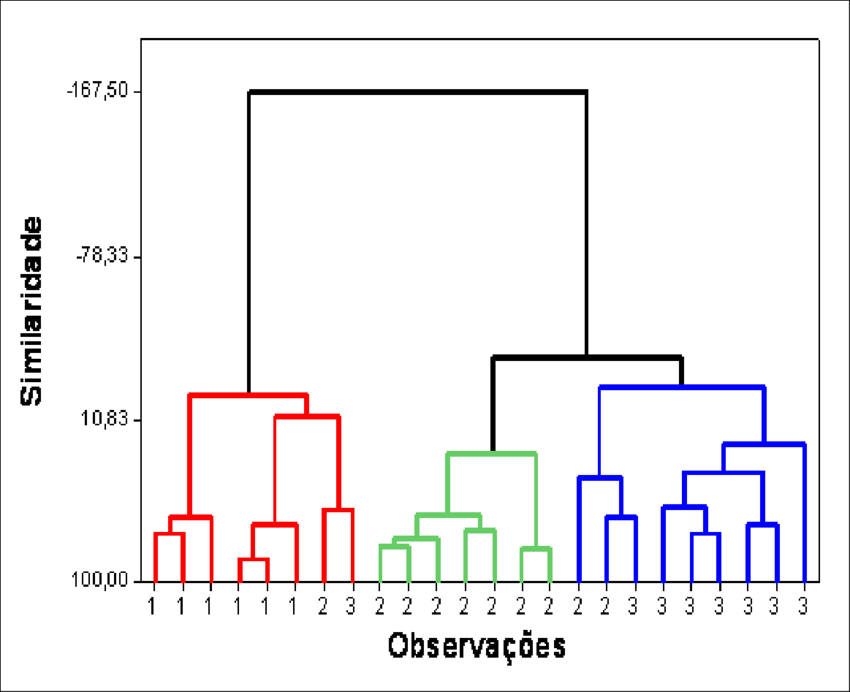
\includegraphics[scale=0.50]{figs/cluster_h.png}
    \caption{Exemplo de agrupamento hierárquico}
    \label{fig:clusterh}
 \end{figure}
 
 \pagebreak
 
 \section{Similaridade em dados textuais}
 Conforme introduzido anteriormente, definir uma métrica de similaridade entre os objetos é essencial para o funcionamento dos algoritmos de clusterização.
 Para o propósito deste trabalho, iremos explorar técnicas que extraem essa similaridade em dados textuais.
 
 Para uma base de dados textual,  utilizaremos o termo \textbf{``texto bruto''}  para se referir ao conteúdo de cada registro na base de dados. 
 Também adotaremos o termo \textbf{documento} para partições dos dados (por exemplo, uma linha da tabela).
 Estenderemos a definição de \emph{palavras} e \emph{separadores} utilizadas no capítulo anterior, definidas sob um ponto de vista linguístico (não relacionados diretamente a notação de conjuntos definida no capítulo ~\ref{chapter:fund}).
 
 \subsection{Vetorização TF-IDF}
Análise de texto é umas das aplicações mais exploradas no campo dos sistemas inteligentes.
Porém, pode ser uma tarefa difícil utilizar texto bruto como entrada para os algoritmos de \emph{machine learning}. 
Geralmente, tais algoritmos ``lidam melhor'' com características numéricas.
 
O processo de transformar documentos em vetores de características numéricas é conhecido como \textbf{vetorização} \cite{Qaiser}. 
Em geral, procuramos uma medida que atribua pesos a cada palavra, de acordo com a sua ``importância'' no documento.

Poderíamos atribuir pesos às palavras de maneira direta e intuitiva, atrelando o peso diretamente a frequência em que aquela palavra ocorre em um documento.
Chamamos esta medida de \textbf{TF} (\emph{term frequency}).

\begin{equation}\label{eq:tf}
tf(t, d) = \frac{count(t \in d)}{count(d)}
\end{equation}

Onde $t$ é a palavra (ou termo) alvo da medição, e $d$ é o documento que contém a palavra $t$  e pertence a coleção de documentos $D$.

Entretanto, algumas palavras (como ``and'' ou ``him'' no inglês) adicionam pouca ou nenhuma informação relevante para o texto em si, apesar de sua alta frequência, essas palavras são conhecidas como \textbf{\emph{stop words}}.
Remover as \emph{stop words} pode diminuir ruídos nos dados utilizados para o modelo de classificação, sendo um recurso muito importante para a construção de clusters com maior significado semântico.

Para compensar este fator, o \textbf{IDF} (\emph{inverse document frequency}) pondera o quão ``incomum'' é um determinado termo entre diferentes documentos, atribuindo valores baixos a termos que se repetem muito em diferentes documentos \cite{Qaiser}.

\begin{equation}\label{eq:idf}
idf(t, D) = \log \frac{len(D)}{count(d \in D : t \in d)}
\end{equation}


A métrica \textbf{TF-IDF} multiplica as equações~\ref{eq:idf} e ~\ref{eq:tf}, de maneira que a informação da frequência de um termo é ponderada pela sua ``exclusividade'' entre os documentos.
Obtemos assim uma métrica que aproxima a zero os símbolos menos relevantes, e atribuí valores maiores a símbolos ``mais relevantes''.

\begin{equation}
tfidf(t, d, D) = tf(t, d) \times idf(t, D)
\end{equation}

 \section{Redução de Dimensionalidade}
 Em casos em que a base de dados possuem uma quantidade elevadas de dimensões, 
reduzir a dimensionalidade significa procurar variáveis que possuem dependência entre si.
No geral, busca-se manter apenas características relevantes aos dados, reduzindo sua complexidade e o poder computacional necessário para processar estes dados.

 \subsection{PCA}
 O PCA (ou \emph{principal component analysis}) é formado por um procedimento algébrico, 
 que reduz as variáveis correlacionadas em um conjunto de variáveis não relacionadas (linearmente) chamadas \emph{principal components} (PCs), iterativamente \cite{Jolliffe}.
 No contexto da clusterização, o PCA é utilizado principalmente para transformar dados com muitas dimensões em uma representação com menores dimensões (usualmente duas dimensões, facilitando a análise gráfica dos dados).
 
 
 \section{Clusterização K-means}
O método de clusterização \emph{k-means} (ou algoritmo de Lloyd's \cite{Lloyd}) é um algoritmo iterativo que particiona os dados em $k$ clusters, definidos por \textbf{pontos centrais} (onde $k$ é uma das entradas para o algoritmo).
A ideia em geral é encontrar os melhores $k$ pontos centrais, isto é, posicionar estes pontos de maneira a minimizar a distância dos dados aos pontos centrais mais próximos. 
Podemos definir o k-means da seguinte forma:
 \begin{enumerate}
 	\item Escolha os $k$ primeiros pontos centrais. A escolha pode ser \textbf{aleatória}, ou utilizando o \emph{k-means++} (algoritmo para inicializar os pontos centrais).
	\item Calcule a distância de cada dado em relação a cada ponto central.
	\item Atribua cada dado ao ponto central mais próximo.
	\item Calcule a distância média entre os pontos e seus respectivos centros para cada cluster, e obtenha novas localizações para os pontos centrais (de maneira a minimizar a distância média).
	\item Repita os passos 2, 3, e 4 até que os clusters não mudem, ou atingir o número máximo de iterações.
\end{enumerate}
 
 \begin{figure}[H]
   \centering
   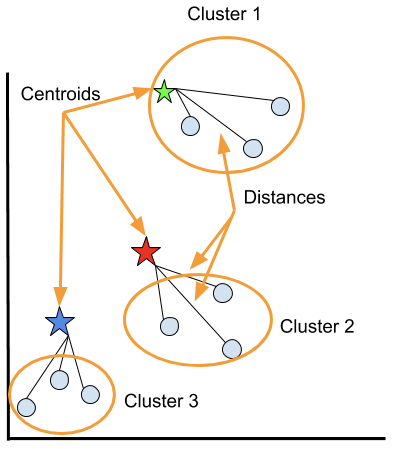
\includegraphics[scale=0.40]{figs/kmeans.png}
    \caption{Exemplo de clusterzacao k-means}
    \label{fig:kmeans}
 \end{figure}
 
 
 \subsection{Método de elbow}\label{ssec:elbow}
 O resultado do \emph{k-means} é diretamente afetado pelo número de clusters definidos na inicialização do algoritmo.
 Existem diversas formas para determinar o número ``ideal'' de clusters, uma delas é o \textbf{método de elbow} \cite{Humaira}.
 
 Neste método, executa-se o \emph{k-means} para um range pré-definido de valores em $k$. 
 Depois disso, calcula-se a soma das distâncias quadráticas (também chamada de \textbf{inércia}) de cada ponto para o seu respectivo ponto central.
 0 resultado para cada $k$ é plotado em um gráfico de linha (conforme mostra a figura~\ref{fig:elbow}).
 Seleciona-se o número de clusters que corresponde ao ``cotovelo'' (elbow) do gráfico.
 
\begin{figure}[H]
   \centering
   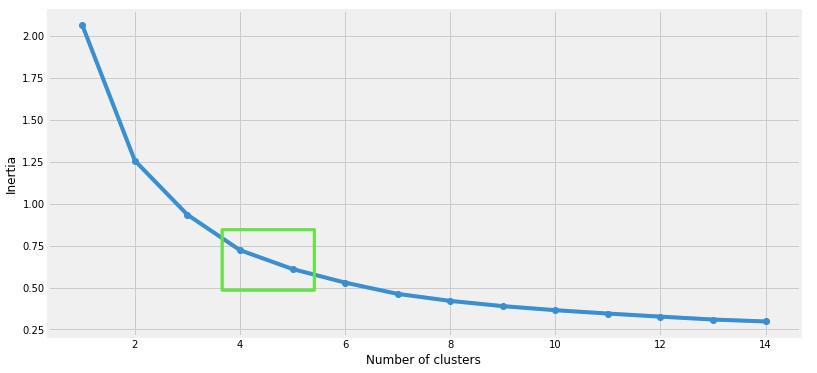
\includegraphics[scale=0.40]{figs/elbowex.png}
    \caption{Método de elbow}
    \label{fig:elbow}
\end{figure}

 
 


